\section{Обзор научной литературы}
\label{cha:review}
\section{Организационная эффективность}
Гуру научного менеджмента Майкл Портер в своей книге "Международная конкуренция: конкурентные преимущества стран" \cite{porter1993m} выделяет эффективность научно-исследовательской работы как один из способов конкуренции стран. 

Существует множество подходов к трактовке понятия эффективности вообще и в научно-исследовательской работе, в частности. Но важно понимать, эффективность - это не коэффициент \cite{tikin2009e}. 

В работе \cite{kle2014o} отмечается, что научно-исследовательская работа не может быть однозначно описана и оценена с использованием унифицированных и объективных показателей продуктивности, что свидетельствует о необходимости использования сразу ряда показателей. 

В статье Левина \cite{levin2016v}, автор выступает против исключительно количественной оценки исследователей. Но несмотря ни на что, тенденция формальной оценки научных исследований продолжает распространяться в связи с отсутствием альтернативы отношению к научным текстам, как к основному продукту, производимому исследователями. При этом сам процесс производства научного текста не рассматривается в деталях в виду его творческой природы и остается ``черным ящиком''. Автор данного исследования видит в этом иррациональность и считают своей обязанностью исследовать сам процесс производства научных текстов как основу для дальнейшей оценки продуктивности научной работы и выявления возможностей для повышения продуктивности исследователей.

К основным компонентам процесса научного исследования относят формирования коллаборации исследователей, процесс создания научной статьи и ее публикации. Опубликованная научная статья является одним из воплощений результатов научного исследования. Существует множество методик ведения исследовательской деятельности. Большинство из них использует структурирование научно-исследовательской деятельности на этапы для упрощения ее понимания. Например, в книге \cite{lipch2013met} выделены следующие семь этапов:
\begin{enumerate}
\tightlist
\item Выбор темы научного исследования.
\item Изучение мирового опыта по выбранной теме посредством научных источников.
\item Составление плана научно-исследовательской работы.
\item Накопление материала для проверки обоснованности выдвинутой гипотезы.
\item Обработка данных, построение моделей.
\item Анализ результатов исследования и выводы.
\item Документальное оформление научно-исследовательской работы.
\end{enumerate}

Таким образом, создание научной статьи, как результат научного исследования, может быть представлено в виде формализованного процесса, реализуемого участниками научно-исследовательской группой. Этот процесс принадлежит к категории коллективного социального взаимодействия. И его изучение является нашей задачей в данном исследовании. Поэтому автор поставил задачу рассмотрения именно процесса совместного проведения научно-исследовательской деятельности и написания научной статьи с последующей публикацией. Кроме этого автор данного исследования постарался учесть процессы коллективного мышления и коммуникаций, отмеченные в работе \cite{mkrt1995f}.

В научной практике исследователи должны делиться результатами своих исследований с коллегами. Публикация статьи в научном журнале является одной из форм коммуникации исследователя с научным сообществом \cite{danil2016o}. Помимо публикации статьи, коммуникация может быть осуществлена в виде публикации монографии, тезисов конференций или патентов, а также личных выступлений на конференциях и семинарах. Поэтому научное исследование не может рассматриваться по мнению автора в отрыве от процесса публикации. Таким образом, в коллаборацию коллектива исследователей необходимо включить редакцию научных журналов и комитеты научных конференций.

В самом упрощенном виде редакции и комитеты конференций группируются не по формальным рубрикаторам, типа ГРНТИ, а по определенным ментальным кодам \cite{gary2016unpacking}, скрытым за описаниями формата и редакционными политиками. Примером такого кода может быть: ``Мы принимаем статьи только от членов SPE (Society of Petroleum Engineers)'' или ``Авторы должны иметь научную степень''. Понятие ментального кода широко применяется при анализе объединения в группы \cite{sidor2006g,gentner2014mental}. 
Ментальный код может состоять из отдельных фрагментов, как молекула ДНК. Важно понимать, что именно на основании совпадения ментального кода производится принятие нового участника в сообщество. Что, в нашем случае, означает принятие редакцией или комитетом конференции научной работы к публикации. Иногда часть ментального кода может быть продекларирована, но это не означает, что существенная его часть, на основании которой и будет приниматься решение не остается внутренним достоянием редакции или программного комитета. В таком случае автор будет испытывать недоумение от того, что ему ``немотивированно'' отказали, так как существенная часть ментального кода редакции или программного комитета конференции ему не доступна.

Процесс публикации научной статьи так же имеет формальные этапы, в которых, однако, не отражен сетевой процесс работы над результатом:
\begin{enumerate}
\tightlist
\item Объявление о дате и теме проводимой конференции;
\item Запрос аннотаций статей (call for papers);
\item Экспертная оценка (peer review);
\item Подготовка текста на двух языках;
\item Создание доклада;
\item Выступление с докладом;
\item Подготовка текста в формате для публикации;
\end{enumerate}

Таким образом, можно говорить о фундаментальном процессе, содержащем логику расширения группы, на основании которого работают как малые группы – соавторы, так и большие группы, включающие в общем случае представителей редакций, организационных комитетов конференций, ``гостевых авторов'', переводчиков, экспертов, осуществляющих оценку и т.п. Рассмотрение таких коллабораций необходимо для понимания процесса публикации научной статьи и последующей оценки вклада отдельных участников.

Разделение труда характеризует зрелость производственных процессов. Для рассматриваемого нами процесса написания научных статей это может означать, что создаются специализированные пулы ресурсов для поддержания определенных этапов без персонификации. Например, из прошлого нам известно жаргонное выражение ``кооператив по вписыванию формул'' применительно к кандидатским диссертациям. Несмотря на маргинальность этого явления, которое публично осуждалось и процветало за счет востребованности в узкой специализации, автор видит в нем ранние предпосылки для разделения труда в процессе производства научного исследования и публикации на его основе. В настоящее время в связи с ускорением производства научных исследований появились новые формы разделения труда (и новые требования к результативности научно-исследовательских кадров), которые нуждаются в изучении.

Вопрос коллективного создания знаний и написания научных исследований в частности имеет много аспектов, связанных с этикой исследователя. Должен ли автор, полностью выполнять все этапы работы над исследованием? Если в работе два соавтора, то какое разделение труда не нарушает этических норм исследователя? Какие роли среди соавторов этичны? В общеизвестном ``Курсе теоретической физики'' Ландау и Лифшица какую роль выполнял Л. Д. Ландау, а какую Е. М. Лифшиц?

После объединения на основе ментального кода происходит развитие отношений в рамках коллабораций в широком (с внешними участниками) и узком (в рамках исследовательской группы) смыслах. Укрепление соавторских отношений в результате написания нескольких работ создает более устойчивые рабочие группы. Существуют примеры продолжающихся на протяжении десятилетий соавторств. С другой стороны, есть примеры, когда, написав одну исследовательскую работу, авторы больше не сотрудничают. В чем причины устойчивых объединений в соавторские коллективы?

Автор считает, что во многих научно-методических источниках основное внимание уделено технологиям написания научной статьи и ее оформлению, но не изучению процесса создания научных статей, поэтому считают данную работу практически полезной для администрирования и планирования НИР в понятиях научного менеджмента по системе Тейлора \cite{taylor2004scientific} .

Проблема объективной оценки эффективности НИР находится в центре внимания исследователей уже давно, и это, в первую очередь, связано с вопросами финансирования как бюджетного, так и в рамках грантов. В рамках традиционного подхода выделяются следующие индикаторы оценки эффективности \cite{korol2014krit}:

\begin{itemize}
\tightlist
\item Финансовые
\item Кадровые
\item Инновационные
\item Библиометрические
\end{itemize}

Собственно в рамках библиометрии учитываются следующие параметры:

\begin{itemize}
\tightlist
\item число публикаций в международных журналах характеризует качество статей; 
\item индикатор цитирования и индекс Хирша показывают степень значимости проводимых исследований и признание научных школ мировым сообществом;
\item ``публикационная нагрузка'' ученых – продуктивность ученых; 
\item наличие патентов; 
\item соавторство с зарубежными учеными – показатель международной кооперации''.
\end{itemize}

Как отмечают многие исследователи \cite{vonortas1995new, veugelers1998collaboration, faems2005interorganizational }, этот набор параметров далек от совершенства, поскольку не даёт полностью объективную картину НИР выбранного учёного или коллектива. Например, индекс Хирша зависит от дисциплины, а также он не спадает, если человек не публиковал новых работ в течение 10 и более лет. Цитатные базы WoS и Scopus, во-первых, неполноценно отражают исследования на русском языке, а во-вторых, разным дисциплинам отводятся в них неравные доли. 
В данном исследовании проверяется гипотеза, что повышение качества оценки эффективности НИР возможно через учёт дополнительных факторов, о которых будет сказано далее.

Эффективность организации – очень сложный и многогранный концепт. 
На него оказывают влияние различные факторы. 
Одним из важных предвестников рыночного успеха научно-исследовательской компании является хорошо развитая коммуникация и кооперация между сотрудниками. 
Многие теоретические и практические исследования демонстрируют связь между продуктивностью организации и структурой коммуникации её сотрудников, например,  в работах  \cite{allen1984managing,noe2006human}.
Исследование социальной структуры организаций и профессиональных сообществ становится одним из главных направлений прикладного анализа социальных сетей. 
В сфере общественных связей и управления глубоко изучаются модели коммуникаций внутри организаций. 
Начало этим исследованием положено в 1956 году работе C.H.Cooley ``Социальная организация'' \cite{cooley1956social}.

Информация о взаимодействиях сотрудников может быть получена различными способами, например, с помощью корпоративных баз данных, общественных опросов и личных отчётов. 
Однако, данные, полученные такими путями, нужно интерпретировать с некоторыми оговорками, поскольку они не отражают всего механизма профессионального взаимодействия в целостности. 
Как утверждают Вассерман и Фауст \cite{wasserman1994social}, около половины того, что люди сообщают о своих взаимодействиях, по той или иной причине неправильно. 
Таким образом, людям не очень хорошо удаётся качественно информировать о своих взаимоотношениях, поэтому пути сбора данных должны избегать такой субъективности.

Источником такой информации может быть Google Scholar, arXiv и другие онлайн библиотеки. 
Рассмотрение открытых научных сообществ так же интересно, как и сужение выборки до одной страны, отрасли и организации. 

Одним из более объективных способов анализа человеческих взаимодействий является формальный концептуальный анализ (англ. formal concept analysis, FCA). 
FCA представляет собой определенный способ анализа коллекции объектов и их свойств. 
Идея применить FCA в области анализа социальных сетей уже не нова. 
В работе \cite{kurtz2009c} он был использован для массового анализа сети. 
В \cite{snasel2009analyzing} комбинация формального концептуального анализа и известных методов факторизации была направлена против вычислительной  сложности анализа социальных сетей, а также на облегчение визуализации этого анализа. 
Би-кластеризация и три-кластеризация были применены в \cite{gnatyshak2012gaining} для анализа данных, собранных в русской социальной интернет-сети Вконтакте для выделения групп пользователей со схожими интересами, для поиска сообществ пользователей, входящих в состав схожих групп и для выявления интересов пользователей. 
Формальный концептуальный анализ многократно использовался для анализа социальных сетей, основанного на ссылках \cite{kuznetsov2007reducing}, 
для обнаружения криминальных сетей \cite{poelmans2012semi}. 
Другие способы применения FCA можно почерпнуть в работе \cite{poelmans2013formal}. 
Весьма подробный анализ приложений на основе FCA для анализа социальных сетей можно найти в \cite{aufaure2013advances, obiedkov2007social, pensa2005towards}.

Одним из частных случаев коммуникации является кооперация, которая может в случае научно-исследовательской работы переходить 
в соавторство при создании научных публикаций. 

Публикация научных исследований – главный объект, по которому оценивается эффективность научно-исследовательской работы. 
Поэтому важно проследить, как проходит этот процесс, начиная с зарождения исследовательской идеи, проведения эксперимента и заканчивая публикацией работы. 
Необходимо провести анализ, какие условия способствуют успешной публикации статьи. 
В рамках данного исследования было изучено соотношение публикаций отдельных учёных и научных коллективов. Было показано, что за последнее десятилетие есть чётко выраженная тенденция ученых объединяться в группы соавторов для публикации статей. 
Отсюда можно сделать вывод, что одним из факторов, положительно влияющих на опубликование работ, является объединение людей в команды.

В свою очередь, командообразование тоже бывает успешным и неуспешным, оно также поддаётся изучению, в результате которого можно выделить условия успешного командообразования. 
Задача поиска оптимальных параметров команды соавторов для наиболее продуктивного написания научных статей относится к классу задач оптимизации. 
Традиционно исследователи обращают внимание на следующие параметры, имеющие значение для продуктивного научного творчества:
\begin{itemize}
\tightlist
\item Размер команды         
\item Ментальные модели сообщества
\item Компетенции сотрудников (дополняющие и гомофильные)
\item Слабые связи между учёными
\end{itemize}

В отличие от размера команды, который является явным, а не скрытым признаком, а также легко формализуемым, 
признак ментальных моделей (англ. mental model) сообщества гораздо труднее поддаётся выявлению и фиксации. 
Многие исследователи отмечают важность изменения во времени ментальных моделей помимо структуры команды \cite{klimoski1994team, morgeson1999structure}. 
Понятие ментальной модели является развитием понятий структуры знания \cite{walsh1995managerial}, схемы знаний \cite{fiske2013social, sims1986thinking}, и неявной теории \cite{brief1983cognitive}. 
Автор данного исследования трактует понятие ментальной модели как стратегическую согласованность командных компетенций. 
Например, ментальная модель ``Agile geoscience'' \cite{hall2011shale} крупнейшего сообщества ученых-геофизиков основывается на компетенциях ``гибкие методики'' и ``геология''.

Исследователи сходятся в том, что совпадение ментальных моделей участников команды положительно влияет на производительность \cite{lim2006team, mathieu2000influence}. 
Этот факт говорит о связи ментальной модели команды и полного командного кода, которое более подробно раскрыто далее. 

Формирование основной системы внутреннего взаимодействия внутри команды согласно исследованию \cite{harper1985power} происходит при знакомстве участников по принципу дополняемости.
Тем не менее, нельзя полностью отрицать значение гомофильных (совпадающих) компетенций. 
Во многих работах отмечается динамическая структура гомофилии \cite{mcpherson2001birds, snijders2010introduction, steglich20108}, в ходе которой параллельно происходят два процесса. 
С одной стороны – схожие между собой индивиды формируют социальные связи (социальная селекция). 
С другой – уже связанные друг с другом люди перенимают поведение друг друга (социальное влияние). 
Совокупность этих факторов результирует в гомогенную социальную систему, 
в которой между индивидами со схожим поведением и характеристиками есть связь, при этом характер связи может быть, как формальным, так и неформальным.                     

Несмотря на то, что связи между индивидами со схожими характеристиками более вероятны, чем связи между непохожими, уровень схожести также важен. 
В работе \cite{block2014multidimensional} было показано, что социальная схожесть более, чем по одному показателю, 
приводит к тому, что люди с меньшей вероятностью будут формировать между собой взаимоотношения. 
Автор объясняет данный эффект тем, что слишком схожие по многим характеристикам люди, как правило, 
не могут привести что-то новое и конструктивное во взаимные отношения или же в команду. 

Для продуктивного сотрудничества необходима не только схожесть интересов, 
но также и различный профессиональный и жизненный опыт, позволяющий предложить многомерные подходы к ее решению.

\section{Место текста в научной деятельности}
Анализ текста иногда называют \textit{Text Mining}. Суть этого процесса в превращении данных (текста) в высоко-качественную информацию способную приносить знания. Важным моментом является то, что при получении знаний человеческие затраты должны быть минимальны. 

Полученные из текста знания становятся основой для принятия управленческих решений в организационной среде. 
Отдельным процессом рассматривается получение текста, иногда называемое созданием корпуса текстов. 

Реальный мир находит свое отражение в текстах при помощи авторов, а процесс анализа текста делает обратное: на основе текстов составляет информацию о реальной природе вещей. 

Многомодовым подходом к анализу текстов называют процесс учитывания сопутствующей основному тексту информации. Например адрес письма, номер выпуска газеты с новостями или фамилии соавторов научной статьи. 

Формально анализ текста производится в следующей последовательности: 
\begin{enumerate}
\tightlist
\item анализ языка текста
\item анализ содержания текста
\item получение информации об авторе текста
\item вывод определенных переменных, характеризующих природу вещей в тексте
\end{enumerate}

Рассмотрим более подробно методы работы с текстами научных статей.

\subsection{Обработка текста}
Задачи по обработке текста были поставлены в 60-70 годах 20-ого века при обработке натурального языка \cite{weizenbaum1966eliza, kuvcera1967computational}.
Нужно было приводить текст к более удобной для последующего анализа форме. Эту процедуру общепринято называть \textit{нормализацией текста}. Для нормализации текста  использовались регулярные выражения (regular expressions), концепцию которых разработал С.К.Клини \cite{kleene1951representation}. Одним из первых, кто использовал регулярные выражения в работе с тестом был К.Томсон \cite{thompson1968programming}.

В настоящее время задачи нормализации текста существенно расширились. Нужно не только выделять слова, но и учитывать специальные символы, обозначающие эмоции (Emoji), такие как 8-) \cite{eisner2016emoji2vec}, выделять хештеги \cite{o2010tweets},  выделять гиперссылки \cite{bingel2017identifying} и обрабатывать цитирования \cite{jha2017nlp}.
	
Задача лексического анализа состоит в разделение текста на части - предложения, слова, буквы.  Иногда лексический анализ называют токенизацией от английского слова \textit{tokenizing} \cite{lovins1968development}.

Другая задача нормализации текста состоит в определении слов с единой основой и называется лемматизацией. Основа слова не обязательно совпадает с морфологическим корнем слова. 
Лемматизация для русского языка отличается от лемматизации для английского \cite{segalovich2003fast, sharoff2011proper, korobov2015morphological}. Поэтому для английского языка используют процедуру лемматизации на основе частотных алгоритмов \cite{willett2006porter, porter2001snowball}, так же называемую стемминг от английского слова \textit{stemming}. Но для других языков лемматизация использует еще более сложные алгоритмы. Например, есть стемминг для Древнегреческого языка \cite{packard1973computer}.

Таким образом нормализация текста состоит из трех этапов: 
\begin{enumerate}
\tightlist
\item Выделения слов из текста
\item Приведения слов к более общим формам 
\item Выделении предложений 
\end{enumerate}

Для автоматизации задач нормализации текста используют библиотеки на языке программирования Python. Например, библиотеку NLTK \cite{bird2009natural}, содержащую огромное количество различных алгоритмов обработки текста.

\subsection{Модели текста}
\label{sec:textmodel}
Модели, которые присваивают вероятности словам в последовательностях слов называются вероятностными моделями текста. Математически это определение можно записать в виде уравнения. 
Допустим у нас есть вероятность последовательности из $n$ слов $ P(w_1, \dots, w_n)$, такая, что вероятность третьего слова $P(w_3) $ равна $P(w_3|w_1,w_2)$. 
Тогда следующее выражение определяет вероятностную модель текста. 

\begin{defi}[О\ref{defi:rev1}] 
\label{defi:rev1}
$$P( w ) = P( w_1, w_2, \dots , w_n ) =  \prod_i^n P( w_i | w_1, w_2, \dots , w_{i-1} )$$
\end{defi}

Так как вычисление $P (w) $ представляет сложность $O^n$, то современные исследования текста используют представление $P ( w )$, как однородной Цепи Маркова и строят приближенные модели \cite{schwenk2002connectionist}: 

\begin{enumerate}
\tightlist
\item Униграмная модель $ P(w_1, w_2, \dots , w_n )  \approx \prod_i P(w_i)$
\item Биграмная модель $ P(w_i \vert w_1, w_2, \dots , w_{i-1} )  \approx  \prod_i P(w_i \vert w_{i-1} )$
\end{enumerate}

Можно так же рассматривать n-грамные модели для большего охвата контекста, как в работах \cite{teahan1996entropy, teahan1997models}. Применительно к задачам распознавания речи это сделано в работах исследователей из ИБМ \cite{bahl1983maximum, bahl1986maximum, averbuch1987experiments}.

Tomas Mikolov в работах \cite{mikolov2013efficient,mikolov2013distributed} показывает, что и эти упрощенные модели обладают слишком большой вычислительной сложностью, поэтому его лаборатория разработала векторное представление слов не с помощью априорных распределений как в исследовании \cite{blei2006dynamic}, а на основе встраиваемых (embedded) векторов. 

Из определения (О\ref{defi:rev1}) следует и способ для проверки качества вероятностной модели текста. Для этого пользуются метрикой \textit{Perplexity}: 

\[ 
\mathcal{P}  = \sqrt[n]{\frac{1}{P(w)}}
\]

В работах \cite{cover1991entropy, algoet1988asymptotic} показано, что между метрикой \textit{Perplexity} и относительной энтропией на одно слово $  H(W)$ существует следующая зависимость: 

\[
 H(W) = \log_2 Perplexity(W) 
\]

Клод Шеннон \cite{shannon1951prediction} оценил энтропию  английского языка как 0.6 - 1.3 бита на букву, прося людей предсказать следующую букву слова. 
В работе \cite{cover1978convergent} дана оценка нижней границы энтропии английского текста как 1.25, а в работе \cite{brown1992estimate} с использованием триграм модели слов приведена оценка 1.75 бит на слово.  

Но есть и другие подходы к оценке качества моделей текста. Например в работах \cite{cohen1998learning, collobert2011natural} использует метрику основанную не на энтропии, а на попарном сравнении (pairwise ranking approach).

Помимо подхода, развиваемого T.Mikolov, существуют и другие способы векторного представления слов. Следует отметить работу исследователей и Университета Стандфорд, названную GloVe \cite{pennington2014glove}. Векторное представление слов Glove требует существенно меньше вичислений, так как использует только частоты употребления слов, а не вероятности.  

\subsection{Классификация текста}
\label{sec:textclassification}
Самым распространенным примером потребности в классификации текстов, наверное, является задача отнесения писем к категории нежелательных почтовых рассылок, называемых спамом. И базовой линией для этой задачи является классификатор на основе алгоритма Наивный Байес (НБ).

Наивная Байесовская текстовая классификация была предложена М.Мароном в работе \cite{maron1961automatic} для присвоения категории принадлежности текста доклада определенному журналу. 
Его модель представила большинство особенностей, используемых и в настоящее время для задач классификации текстов. 

Байесовские методы \cite{bayes1763essay} были также применены к задачам классификации текстов по авторству в пионерской работе Ф.Мостеллера и Д.Уоллеса \cite{mosteller1963inference}. 
Наивный Байес был впервые применен для обнаружения спама в работе \cite{sahami1998bayesian}.

В работах \cite{metsis2006spam, wang2012baselines, pang2002thumbs} было показано что, использование бинарных признаков с мультиномиальным распределением дает лучшие результаты, чем счетчики слов. 

Бинарный Байес с Мультиномиальным распределением часто путают с другим вариантом наивных Байесовских алгоритмов, которые также используют двоичное представление того, встречается ли слово в документе: Многовариантный Наивный Байес (МНБ) с использованием распределения Бернулли. 
Вариант НБ с рапределением Бернулли оценивает вероятность того, что слово не входит в документ. 

В исследовании \cite{mccallum1998comparison} показано, что МНБ не всегда хорошо обобщается на новые тексты.

Задача определения эмоциональности текста относится к задачам классификации и успешно решается с помощью алгоритмов НБ.  
Существует ряд хороших обзоров применения анализа эмоциональности текстов среди которых работы \cite{pang2008opinion, liu2012survey, stamatatos2009survey}.

Стоит также отметить хороший обзор различных текстовых классификаторов, сделанный К.Маннингом с соавторами \cite{schutze2008introduction}.

В настоящее время векторное представление частей текста (embedding)
приобрело большую популярность. Широко используются методы Word2Vec
\cite{mikolov2013efficient}, GloVe \cite{pennington2014glove},
StarSparse \cite{wu2017starspace}, Fasttext \cite{bojanowski2016enriching}, Sent2vec
\cite{pagliardini2017unsupervised}. 
Поэтому стоить упомянуть и рациональный взгляд на преимущества
от использования векторного представления  

Основной демонстрацией преимущества от использования векторного
представления слов стала формула: king - men = queen.
Смысл этой формулы в том, что векторные представления слов (king, men, queen) можно подвергать арифметическим операциям. 

Но отнюдь не все слова так складываются. Некоторые очевидные для человека аналогии в векторном представлении не являются близкими векторами \cite{finley2017analogies}.
Поиск смыслов в векторных представлениях предпринят в работе \cite{pelevina2017making,panchenko2017unsupervised}.

Алгоритм AdaGram предложен в работе \cite{bartunov2016breaking} для  поиска векторных представлений для неоднозначных слов.
Исследование уточнения пониманий векторных представлений в зависимости от контекста предпринято в работах \cite{huang2012improving,gladkova2016intrinsic}. 
 
Существенные преимущества в классификации текстов были получены от применения рекуррентных нейронных сетей. 
Из всей массы работ в этом направлении необходимо отметить многочисленные исследования текстовых моделей на основе нейронных сетей
выполненные сотрудниками лаборатории естественного языка при Стенфордском университете \cite{schuster2018gapping,eric2017copy,wang2017naturalizing,li2017adversarial,xie2017data}.

\section{Анализ социальных сетей}

В книге \cite{de2018exploratory} отмечается, что базисом для анализа социальных сетей является теория социометрии, основанная J.L.Moreno \cite{moreno1953shall}. 
Социометрия изучает взаимоположения социальных атомов в группах. 
Социограммой по Морено является графическое отображение социального выбора членов социальной группы.
Социальным выбором может быть выбор лидера, дружба, выполнение совместных задач, и др. 
Социограма представляет граф, состоящий из вершин и ребер. 

В книге \cite{tsvetovat2011social} M.Tsvetovat  с соавторами ставит вопрос:
Кто из участников организации, представленной в виде графа, важнее? 
Таким образом проводя логическую связь между графами и организационной теорией, что отмечено в работе \cite{atherley2015model}.

Хорошим примером измерения инновационности организации с помощью анализа социальных связей служат исследования \cite{porter2018mapping} .

Направление углубленного изучения графов (Social media mining) деятельных сообществ развито в работах \cite{kurmukov2016classification,zafarani2014social}. Таким образом, переводя различные метрики графов в свойства для задач классификации составляющих графы вершин и ребер. 

Например, в работе \cite{makarov2016co}  метрики графа соавторства использованы для предсказания новых соавторств.
А в работе \cite{makarov2018recommending} предсказание соавторств использовано для повышения эффективности научной организации.

Для решения задач предсказания вершин и ребер графов необходимо рассмотреть, как создаются графы.
Известны модели Small World \cite{watts1998collective}, Preferential Attachment Model \cite{barabasi1999emergence}, и другие модели случайных графов, состоящих из подграфов.

В работе \cite{fortunato2010community} показано, что выделение подграфов дает возможность выявления социальных подгрупп, объединенных общей темой. 
Определение таких сообществ не представляется возможным без использования матетамического аппарата теории графов \cite{lancichinetti2009community}. 

Одной из методик для выявлении сообществ является построения векторного пространства узлов (node embedding) \cite{zheng2016node}. Так же как и с векторным пространством частей текста, описанным в разделе \ref{sec:textclassification}, построение векторного пространства узлов позволяет вводить авторам исследования \cite{liu2017semantic} новые свойства графов на основе близости узлов в векторном пространстве.

Граф соавторства является частным случаем социальной сети. 
Одним из первых исследований графа соавторства является работа \cite{mullins1973development}, сделанная в 1973 году.
С этого времени исследования научной деятельности при помощи графов соавторства не прекращались и обрели статус проверенного инструмента анализа. 
Например, в недавнем исследовании \cite{chuan2018link} предпринята попытка предсказания будущих научных исследований на основе графа соавторства, а в работе \cite{chen2017building} построен глобальный граф соавторства на основе Google Scholar, который содержит более 400 тысяч вершин. Оба исследования проведены в 2017 году.

Построение графа соавторства выполняется таким образом, что если два автора сделали совместную научно-исследовательскую работу, то каждый из авторов считается вершиной графа, а факт соавторства ребром графа. 
Будем называть такой способ создания графа соавторств традиционным. 
В результате такого, традиционного подхода получают граф, изображенный на рисунке (Рис. \ref{fig:rev1}).

\begin{figure}[H]
  \centering
  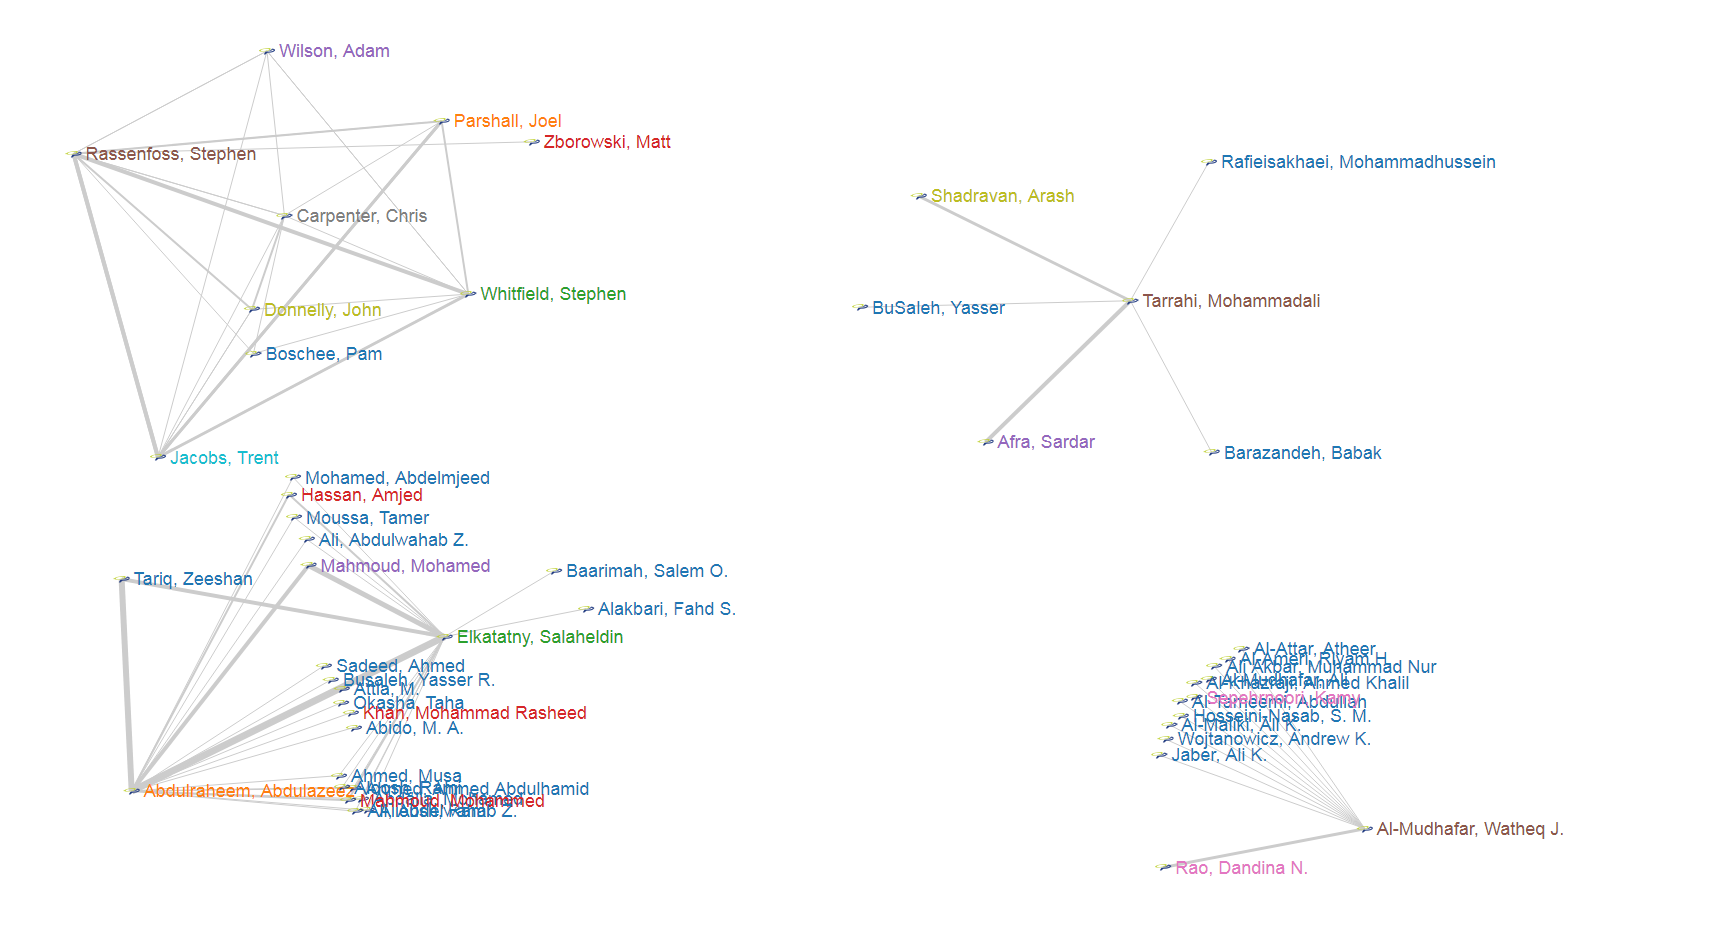
\includegraphics[width=0.8\textwidth]{rev1}
  \label{fig:rev1}
  \caption{Пример простого графа соавторства.}
\end{figure}
